\documentclass[runningheads,12pt]{llncs}
\usepackage{graphicx}
\usepackage{todonotes}
\usepackage{fancyhdr}
\usepackage{lipsum}
\usepackage{tabularx}
\usepackage{array}
\usepackage{longtable}
\usepackage[T1]{fontenc}
\usepackage[provide=*,english,polish]{babel}

\newcolumntype{C}[1]{>{\centering\arraybackslash}m{#1}}

\setcounter{tocdepth}{4}
\setcounter{secnumdepth}{4}
\renewcommand{\headrulewidth}{0pt}

\begin{document}

\title{Współdzielenie kodu w mikroserwisach} \subtitle{}

\author{Artem Romanenko \ Student number: S32237 \inst{}}
\authorrunning{ }
\titlerunning{Your thesis title abbreviated.}
\institute{\textbf{Polish-Japanese Academy of Information Technology} \ Promotor pracy magisterskiej: Krzysztof Barteczko, PhD}

\thispagestyle{fancy}

\begin{figure}[t!]
    \centering
    
\includegraphics[width=\linewidth]{images/Logo_EN_1.png}
    \label{fig:my_label}
\end{figure}

\selectlanguage{english}
\cfoot{ Warsaw, \today}

\clearpage

\makeatletter
\renewcommand*\l@author[2]{}
\renewcommand*\l@title[2]{}
\makeatletter

\selectlanguage{english}
\begin{abstract}
Rapid development and adoption of microservices architecture in last few years changed the world of Informatics. Microservices architecture has many advantages, such as flexibility, fast and comfortable deployment, and easy maintenance. However, this architecture also causes new challenges, such as code duplication and complicated code management. In my master's thesis, I've carried on deep and detailed analysis of all available approaches to manage shared code in system of microservices. In my work, I want to compare all available approaches of code share code in system of microservices using literature sources and prepared code laboratory, also to define cases in which it is better to choose one or another approach. In my practical part, I want to present my own approach to sharing code that will combine the advantages of all existing solutions and provide the best performance and code comfort for developer in code management. At the end of my work, I will place comparison of my solution with existing solutions using prepared performance tests.
\keywords{Microservices Architecture \and Code Sharing \and Performance.}
\end{abstract}

\newpage

\selectlanguage{polish}
\begin{abstract}
Szybki rozwój i powszechne przyjęcie architektury mikroserwisowej w ostatnich latach zmienił świat informatyki. Architektura mikroserwisowa ma wiele zalet, takich jak elastyczność, łatwe wdrożenia i prostota w utrzymaniu. Natomiast powoduje nowe wyzwania, takie jak, na przykład, problem duplikacji kodu i zarządzanie kodem. W mojej pracy magisterskiej przeprowadziłem dokładną analizę metod i podejść współdzielenia kodu w systemach mikroserwisów. W mojej pracy chcę porównać za pomocą źródeł literaturowych oraz przeprowadzonych badań dostępne metody współdzielenia kodu, zdefiniować przypadki w których warto wybrać takie lub inne podejście. Oraz w części praktycznej chcę zaproponować własne nowoczesne podejście do współdzielenia kodu które połączy zalety istniejących rozwiązań i zapewni wydajność oraz komfort w zarządzaniu kodem. Na końcu pracy znajduje się porównanie mojego rozwiązania z istniejącymi za pomocą przygotowanych testów wydajnościowych.
\keywords{Architektura mikrousług \and Współdzielenie kodu \and Wydajność.}
\end{abstract}

\newpage

\tableofcontents

\newpage

\section{Wstęp}

\subsection{Zakres pracy}
W pracy magisterskiej przeprowadzono dokładną analizę metod i podejść do współdzielenia kodu w systemach mikroserwisów, zakres tej pracy zawiera porównanie między architekturą monolitową a mikroserwisową, identyfikację typów obiektów wykorzystywanych w kodzie współczesnych aplikacji, analizę dostępnych metod i podejść do współdzielenia kodu IDL, SDK oraz biblioteki, praktyczna implementacja aplikacji wspierającej nowatorskie podejście do współdzielenia kodu ServerLess.

\subsection{Motywacja}
Główną motywacją do napisania pracy było rosnące w współczesnych czasach zainteresowanie mikroserwisowym podejściem do architektury, które ma wiele zalet, takich jak elastyczność, łatwość wdrożenia i utrzymania na produkcji, możliwość łatwej i szybkiej naprawy problemów na produkcji ale natomiast ma również powoduje nowe wyzwania, takie jak problem duplikacji kodu i zapotrzebowanie na współdzielenie kodu między mikroserwisami w systemie.

W mojej pracy chcę przeanalizować jakie metody współdzielenia kodu są dostępne na rynku, jakie są ich zalety i wady, jakie są najlepsze praktyki w współdzieleniu kodu w systemach mikroserwisów. Porównać bardziej tradycyjne podejścia do współdzielenia kodu, takie jak IDL, SDK, biblioteki z nowatorskim podejściem do współdzielenia kodu takich jak ServerLess, chcę stworzyć oprogramowanie które połączy główne zalety tradycyjnych metod współdzielenia kodu z zaletami bardziej nowoczesnych podejść.

\newpage

\subsection{Zawartość pracy}
Praca jest ustrukturyzowana w kilka rozdziałów, które wprowadzają czytelnika najpierw w szczegóły teoretyczne a później w praktyczne aspekty współdzielenia kodu w systemach mikroserwisów. Krótki opis rozdziałów znajduje się poniżej:
\begin{enumerate}
    \item Wstęp - W tym rozdziale analizuję wady i zalety architektury mikroserwisowej, monolitycznej, porównuję dlaczego z architektury monolitycznej powstała architektura mikroserwisowa, analizuję przypadki w których lepiej użyć architektury monolitycznej a w której architekturę mikroserwisową. Opisuję dlaczego powstało zapotrzebowanie na współdzielenie kodu. Wyjaśniam logikę leżącą u podstaw eksploracji wielu metod współdzielenia kodu. Uzasadniam informację przykładami z literatury.
    \item Architektura mikroserwisowa a Monolitowa - W tym rozdziale porównuję architekturę mikroserwisową z monolityczną, przedstawiam różnice w utrzymaniu i skalowalności, za pomocą źródeł literaturowych prezentuję.
    \item Analiza dziedziny problemowej - W tym rozdziale pracy kategoryzuję typy obiektów które mogą potrzebować współdzielenia kodu w systemie mikroserwisów, analizuję możliwe wyzwania związane z współdzieleniem poszczególnych typów obiektów, przedstawiam uzasadnienia z literatury.
    \item Analiza metod współdzielenia kodu - W tym rozdziale kompleksowa analiza istniejących metod współdzielenia kodu w systemach mikroserwisów za pomocą źródeł literaturowych kryterium ocenia.
    \item Opis części praktycznej - Zawiera opis przygotowanej w ramach pracy aplikacji która wspomaga nowoczesne rozwiązanie do współdzielenia kodu w systemach mikroserwisów - Server Less rozszerzając możliwości tego rozwiązania.
\end{enumerate}

\newpage

\section{Architektura mikroserwisowa a monolitowa}

Rozwój architektury mikroserwisowej w ostatnich latach przyniósł wiele korzyści, takich jak łatwość skalowania, niezależność wdrożenia i elastyczność. Jednak, wraz z tą elastycznością, pojawiają się również nowe wyzwania, związane między innymi z odpowiednim współdzieleniem obiektów pomiędzy mikroserwisami.

\subsection{Architektura mikroserwisowa}

Podział aplikacji na mniejsze, niezależne serwisy umożliwia elastyczne skalowanie poszczególnych komponentów, co przekłada się na lepszą wydajność i dostępność systemu. Ponadto, rozbudowa i utrzymanie aplikacji w oparciu o mikroserwisy jest znacznie prostsza, ponieważ każdy serwis może być rozwijany niezależnie. Taka modularna struktura pozwala na szybsze wprowadzanie nowych funkcjonalności oraz łatwiejsze naprawianie błędów. Istotną korzyścią jest również możliwość korzystania z różnych technologii w poszczególnych serwisach, co daje większą elastyczność i umożliwia wykorzystanie najlepszych narzędzi dla każdej części aplikacji. W rezultacie, architektura mikroserwisowa umożliwia bardziej efektywne zarządzanie projektem, lepszą skalowalność zespołu oraz izolację błędów, co przyczynia się do wyższej jakości i niezawodności systemu.

\begin{quote}
    "Microservices are small, autonomous services that work together. Let’s break that definition down a bit and consider the characteristics that make microservices different."~\cite[p. 2]{newman2015building}
\end{quote}

Charakterystyka architektury mikrousług:
Modułowość - Usługi są modułowe, co umożliwia łatwiejszy rozwój, konserwację i skalowalność, ponieważ każda usługa kontroluje określoną funkcję lub cechę.
Solidność - Mikrousługi zwiększają ogólną solidność systemu, ponieważ błędy w jednej usłudze nie wpływają na całą aplikację, zapewniając tolerancję błędów i niezawodność systemu.
Interoperacyjność - Różne mikrousługi komunikują się za pośrednictwem dobrze zdefiniowanych interfejsów API, zapewniając bezproblemową integrację i interakcję usług.
Równoległy rozwój - Oddzielne zespoły programistyczne mogą pracować nad różnymi mikrousługami jednocześnie, co przyspiesza rozwój i funkcje.
Elastyczność w zakresie elastycznych technologii - Różne mikrousługi można budować przy użyciu różnych technologii, co pozwala na wykorzystanie najskuteczniejszych narzędzi dla każdej przydzielonej funkcji/cechy.~\cite{sharma2023monolithic}

\subsection{Architektura monolitowa}

Architektura monolityczna, która opiera się na jednym spójnym kodzie źródłowym, oferuje pewne korzyści w kontekście prostoty zarządzania i łatwości wdrożenia. Wszystkie komponenty aplikacji są ze sobą ściśle powiązane, co ułatwia debugowanie i śledzenie błędów. Ponadto, brak konieczności konfigurowania i zarządzania infrastrukturą dla wielu usług upraszcza proces wdrażania. W przypadku mniejszych projektów o prostszych wymaganiach, architektura monolityczna może być bardziej efektywna i wydajna, eliminując niepotrzebną złożoność komunikacji między usługami. Jednak warto pamiętać, że architektura monolityczna może napotkać trudności w skalowaniu i utrzymaniu w przypadku większych, bardziej złożonych systemów.

Charakterystyka architektury monolitycznej:
Pojedyncza jednostka wdrożenia - Cała aplikacja jest wdrażana jako pojedyncza, niepodzielna jednostka. Wszelkie uaktualnienia, ulepszenia lub modyfikacje wymagają wdrożenia całej aplikacji, w tym wszystkich jej komponentów.
Scentralizowany przepływ kontroli - Centralny moduł lub funkcja podstawowa nadzoruje przepływ kontroli w aplikacji, koordynując sekwencyjny postęp wykonywania od jednego komponentu do następnego.
Ścisłe sprzężenie - Komponenty i moduły w aplikacji są silnie powiązane i zależne od siebie.
Współdzielona pamięć - Wszystkie komponenty oprogramowania mają bezpośredni dostęp do zasobów pamięci, co sprzyja ścisłej integracji. Jednak taka konfiguracja może również powodować konflikty zasobów i trudności ze skalowaniem aplikacji.~\cite{sharma2023monolithic}

\subsection{Porównanie}

W współczesnym świecie programowania, zawsze wybieramy między podejściem monolitycznym i mikroserwisowym, to wiąże się z kompromisem między prostotą, główną cechą podejścia monolitycznego a elastycznością w przypadku podejścia mikroserwisowego. Podejście monolitowe, które polega na przechowywaniu wszystkich komponentów systemu w jednym miejscu, oferuje łatwość w rozwoju i zarządzaniu kodem ale natomiast może stać wąskim gardłem kiedy aplikacja urośnie. W przeciwieństwie do architektury monolitowej, architektura mikroserwisowa dekomponuje aplikacje w małe, niezależnie zarządzane i wdrażane mikrousługi, umożliwiające granularną skalowalność i niezależne aktualizacje, zmniejszając w ten sposób ryzyko tego, że zmiana w jednym module spowoduje awarię innych. Natomiast takie podejście dodaje skomplikowaności projektom poprzez zapotrzebowanie na obsługę komunikacji między mikroserwisami, wersjonowaniem, współdzieleniem kodu.

\begin{quote}
    "I should call out that microservices are no free lunch or silver bullet, and make for a bad choice as a golden hammer. They have all the associated complexities of distributed systems."~\cite[p. 11]{newman2015building}
\end{quote}

Zalety architektury monolitycznej:
Czas napisania aplikacji - W przypadku małych i średnich aplikacji budowanie aplikacji z architekturą monolityczną jest łatwiejsze i szybsze. Zespół programistów może pracować efektywniej z ujednoliconą bazą kodu bez konfigurowania i zarządzania komunikacją między usługami.
Łatwe wdrożenie - Wdrożenie architektury monolitycznej obejmuje wdrożenie pojedynczej jednostki, co jest mniej złożone i wymaga mniejszej liczby katalogów konfiguracyjnych niż systemy rozproszone.
Uproszczone testowanie i debugowanie - O wiele łatwiejszym jest testowanie aplikacji monolitycznej. Ze względu na ścisłą integrację wszystkich komponentów, testy jednostkowe i integracyjne można przeprowadzać w ramach pojedynczej bazy kodu, co upraszcza proces testowania.
Skalowalność - Architektura monolityczna, w przypadku małych i średnich aplikacji, zapewnia odpowiednią skalowalność poprzez replikację całej aplikacji.~\cite{sharma2023monolithic}

Zalety architektury mikroserwisowej:
Skalowalność - Mikrousługi umożliwiają niezależne skalowanie różnych usług w oparciu o ich zapotrzebowanie, optymalizując wykorzystanie zasobów i zapewniając wydajną wydajność nawet podczas szczytów ruchu.
Utrzymanie kodu - Mikrousługi umożliwiają równoległy rozwój przez różne zespoły, co prowadzi do szybszego rozwoju funkcji i szybszego wdrażania.
Elastyczność w trakcie wyboru technologii - Każda mikrousługa może być rozwijana przy użyciu najbardziej odpowiedniego stosu technologicznego dla jej konkretnej funkcji, co promuje elastyczność i adaptowalność do różnych technologii w ramach tej samej aplikacji.
Łatwe debugowanie - Lokalizowanie i rozwiązywanie błędów w poszczególnych usługach jest proste.
Bezpieczeństwo - Mikrousługi ułatwiają separację danych. Każda usługa ma swoją bazę danych, co utrudnia hakerom próbę naruszenia aplikacji.~\cite{sharma2023monolithic}

Wybór między architekturą monolityczną a mikroserwisową zależy od wielu faktorów, takich jak rozmiar projektu, zapotrzebowanie na ciągły rozwój, wymagania dotyczące skalowalności oraz kompetencje i doświadczenia zespołu. Architektura monolityczna lepiej pasuje dla małych i mniej skomplikowanych projektów natomiast mikroserwisowa oferuje benefity w przypadku wykorzystania w większych, bardziej skomplikowanych systemach.

\newpage

\section{Analiza dziedziny problemowej}

Celem niniejszej pracy magisterskiej jest zgłębienie tematu współdzielenia obiektów w systemach mikroserwisów oraz zrozumienie wyzwań i możliwości związanych z tym zagadnieniem. Praca ma na celu analizę różnych strategii, narzędzi i metodyk, które mogą pomóc w efektywnym i bezpiecznym współdzieleniu danych i obiektów w skali mikroserwisowej architektury.

\subsection{Typy obiektów w aplikacjach mikroserwisowych}

Postanowiłem rozpocząć analizę dziedziny problemowej od tego że za pomocą źródeł literaturowych zidentyfikuję typy obiektów oraz dokonać analizy tego, które z nich mogą wymagać współdzielenia w systemach mikroserwisów.

\begin{enumerate}
    \item DTO (Data Transfer Object) - Takie obiekty są specjalnie przeznaczone do obsługi przesyłania danych między elementami systemu mikroserwisów, są lekkie i nie zawierają logiki biznesowej, dlatego współdzielenie takich obiektów jest jak najbardziej zalecane ponieważ zapewniają spójność danych po obu stronach komunikacji oraz zmniejsza ilość błędów w przypadku rozwoju lub utrzymania aplikacji.
    \item Model (lub Encja) - Najczęściej są logicznie powiązane z tabelami w bazie danych, ze względu na to że we współczesnych czasach za dobrą praktykę jest uważane podejście w którym jeden mikroserwis jest powiązany z maksymalnie jedną bazą danych, współdzielenie tego typu obiektów nie jest zalecane.
    \item Wyjątek (Exception) - Zalecanym jest współdzielenie informacji o wyjątkach w systemie mikroserwisów tym samym tworząc jednolitą obsługę błędów w systemie. Logika związana z obsługą błędów, w przypadku podobności w kilku serwisach też jest dobrym kandydatem do współdzielenia. Taka standaryzacja w systemie mikroserwisów sprawia że łatwiej później znaleźć źródło błędu i naprawić go.
    \item Walidatory - W przypadku współdzielenia walidatorów w systemie mikroserwisów można zapewnić integralność danych w całym systemie oraz zmniejszyć duplikację kodu, również standaryzacja walidacji obiektów w systemie zmniejsza ilość ewentualnych problemów w trakcie ewolucji i rozwoju mikroserwisów w przyszłości, współdzielenie takich obiektów jest dobrą praktyką i jest zalecane.
    \item Serwisy - W przypadku logiki która powtarza się w dwóch i więcej serwisach zalecanym jest współdzielenie takiego serwisu za pomocą najlepiej w tym przypadku pasującej metody, zmniejsza to duplikację kodu natomiast zwiększa czytelność i spójność kodu w systemie mikroserwisów, zmniejsza ilość ewentualnych problemów w trakcie ewolucji i rozwoju kodu.
\end{enumerate}

Zawsze należy pamiętać w trakcie developmentu aplikacji, że współdzielenie kodu ma wiele zalet, natomiast nadmierne współdzielenie kodu może spowodować nadmierne powiązania między mikroserwisami i utrudnić niezależną ewolucję poszczególnych serwisów oraz zniweczyć zalety infrastruktury mikroserwisowej. Również nadmierne współdzielenie kodu utrudnia testowanie aplikacji co może spowodować zmniejszenie jakości kodu. Również nadmierne współdzielenie kodu może spowodować błędy kaskadowe, czyli błędy które pojawiają się w kilku miejscach w systemie jednocześnie spowodowane współdzielonym kawałkiem kodu, utrudnia utrzymanie aplikacji również są powodem na to, żeby podchodzić do współdzielenia kodu ostrożnie podejmować przemyślaną decyzję w każdym konkretnym przypadku.

\newpage

\subsection{Kryteria porównania i analizy metod współdzielenia kodu}

Po przeprowadzeniu dogłębnej analizy tematu i między innymi źródeł literaturowych, takich jak ~\cite{newman2015building}, ~\cite{richardson2018microservices}, ~\cite{nygard2008release}, ~\cite{kleppmann2017designing} mogę zdefiniować kryteria porównania metod współdzielenia kodu w systemach mikroserwisów jako następujące:

\begin{enumerate}
    \item Komunikacja - Metoda współdzielenia obiektów powinna uwzględniać efektywną komunikację między serwisami. Ważne jest, aby obiekty były dostępne w sposób, który minimalizuje opóźnienia i obciążenie sieci. Dobre rozwiązania mogą obejmować użycie asynchronicznej komunikacji, takiej jak kolejki wiadomości, czy też bezpośrednie zapytania między serwisami.
    \item Izolacja - Metoda współdzielenia obiektów powinna zapewniać odpowiednią izolację między serwisami. Każdy serwis powinien mieć kontrolę nad swoimi własnymi obiektami i nie powinien być zależny od innych serwisów. To pozwala na większą elastyczność i umożliwia niezależny rozwój i skalowanie serwisów.
    \item Bezpieczeństwo - W przypadku współdzielenia obiektów, istotne jest zapewnienie odpowiedniego poziomu bezpieczeństwa. Dostęp do obiektów powinien być kontrolowany i zabezpieczony w sposób, który zapobiega nieautoryzowanemu dostępowi. Mechanizmy uwierzytelniania i autoryzacji powinny być odpowiednio wdrożone, aby zapewnić bezpieczne współdzielenie obiektów.
    \item Skalowalność - Metoda współdzielenia obiektów powinna być skalowalna. System powinien być w stanie efektywnie obsługiwać rosnącą liczbę żądań i zapewniać odpowiednią wydajność. Współdzielenie obiektów powinno być projektowane w taki sposób, aby możliwe było łatwe skalowanie poszczególnych serwisów bez wpływu na cały system.
    \item Wersjonowanie - Ważne jest również odpowiednie zarządzanie wersjami obiektów, szczególnie w środowisku mikroserwisów, gdzie różne serwisy mogą używać różnych wersji obiektów. Metoda współdzielenia obiektów powinna uwzględniać zarządzanie wersjami i umożliwiać aktualizacje w sposób kontrolowany i bezpieczny.
\end{enumerate}

\newpage

\section{Analiza metod współdzielenia kodu}

We współczesnych czasach współdzielenie kodu jest niezbędne w skomplikowanych systemach mikroserwisów, w tym rozdziale pracy porównuję istniejące podejścia do współdzielenia kodu oraz porównam je za pomocą zdefiniowanych w poprzednim rozdziale kryteriów. Głównym celem jest zdefiniowanie najlepszych praktyk współdzielenia kodu, zdefiniować, które podejście najbardziej dopasowane do współdzielenia konkretnych typów obiektów, zdefiniowanych powyżej w tej pracy oraz porównanie wydajności i możliwości skalowania w przypadku każdego z podejść za pomocą przygotowanych programistycznych testów wydajnościowych.

\subsection{Metody współdzielenia kodu z opisem}

Za pomocą źródeł literatury oraz własnego doświadczenia zdefiniowałem dostępne na dzień dzisiejszy podejścia:

\begin{enumerate}
    \item Interface definition languages - do IDL należą wiele popularnych technologii, Protocol buffers, Avro IDL, Open API. ~\cite{wiki:interface_description_language}
    \item Libraries - najbardziej oczywiste podejście, które daje możliwość współdzielenia wszystkich rodzajów obiektów w aplikacji.
    \item Client Libraries -
    \item Wyniesienie kodu do osobnego REST serwisu - podejście polega na przechwytywaniu i udostępnieniu wspólnej logiki poprzez utworzenie osobnego mikroserwisu.
    \item Serverless - nowoczesne podejście do pisania kodu i przetwarzania informacji wykorzystywane w chmurach obliczeniowych. Pozwala na uruchamianie kawałków kodu, metod i funkcji niezależnie, bez warstwy zarządzania aplikacją, a także na uruchamianie kodu bez konieczności zarządzania podstawową infrastrukturą. ~\cite{ibm_serverless}
\end{enumerate}

Pryncypia działania poszczególnych metod współdzielenia kodu:

Interface definition languages – są powszechnie używane w oprogramowaniu zdalnych wywołań procedur. W takich przypadkach maszyny po obu stronach łącza mogą używać różnych systemów operacyjnych i języków programowania. IDL oferują most pomiędzy dwoma różnymi systemami. Natomiast również mogą być użyte dla generacji obiektów lub kodów w systemach mikroserwisów. Każdy system IDL posiada określony przez twórców język IDL oraz interpretator języka IDL. Interpretator języka IDL przygotowany i dostarczony przez twórców potrafi na podstawie udostępnionych reguł wygenerować kod używając przygotowane pliki IDL. Używając języka IDL możemy przygotować obiekty lub kod zapisany za pomocą języka IDL, a później udostępnić przygotowane pliki IDL nieograniczonej ilości mikroserwisów i na podstawie udostępnionych plików wygenerować w każdym z mikroserwisów kod lub obiekty, które zostaną użyte przez specyficzną logikę konkretnego serwisu dla osiągnięcia konkretnego celu biznesowego. Tworzenie kodu na podstawie plików IDL jest łatwo zautomatyzowane za pomocą narzędzi do budowania aplikacji, takich jak Gradle czy Maven, dlatego możemy używać IDL jako metodę współdzielenia kodu. W trakcie pracy zamierzam sprawdzić skuteczność tej metody, problemy związane z jej użyciem oraz określić przypadki, w których dobrze się nadaje, jak również przypadki, w których lepiej jej nie stosować.

Libraries – biblioteki to w odpowiedni sposób przygotowany kod, który my za pomocą odpowiednich narzędzi możemy łatwo importować i używać jako część innego programu. Program importujący bibliotekę może używać kodu biblioteki tak, jakby to był własny kod programu. Istnieje wiele narzędzi, które wspomagają łatwe i szybkie importowanie i zarządzanie bibliotekami kodu, takie jak Maven czy Gradle. W współczesnych systemach mikroserwisów współdzielenie kodu za pomocą bibliotek kodu odbywa się za pomocą serwisów do przechowywania artefaktów i plików binarnych, takich jak Nexus. ~\cite[5]{labouardy2021pipeline} Na pierwszym etapie narzędzie do budowania projektu przygotowuje bibliotekę i wysyła ją na serwer. Dalej kod może być przechowywany nieograniczoną ilość czasu na serwerze. Aplikacje, które mają dostęp do serwera, mogą pobrać bibliotekę z kodem i przechowywać w lokalnym systemie plików, używając jako część kodu źródłowego. Biblioteka może być udostępniona nieograniczonej liczbie projektów. Organizacja może ograniczać dostęp do serwera.

SDK – mechanizm działania podobny do bibliotek, różni się jedynie podejściem. W przypadku kodu SDK na serwerze udostępniającym dependencje przechowywane są jedynie obiekty, które muszą być użyte do komunikacji z innym programem lub kodem. Logika biznesowa nie została udostępniona w takim przypadku i zostaje ukryta oraz nie może zostać zmieniona. W przypadku udostępnienia SDK możemy łatwo zapewnić bezpieczeństwo kodu (użytkownicy wciągający dependencje nie widzą logiki biznesowej) oraz chronimy się przed przypadkowymi oraz niepożądanymi zmianami kodu. Pozwala to zaoszczędzić na testach manualnych oraz automatycznych kodu. Przykład, w którym możemy użyć współdzielenia kodu SDK to – mamy mikroserwis, który udostępnia API. API przyjmuje obiekty JSON, które mogą być opisane za pomocą obiektów Java. Obiekty, które pozostałe mikroserwisy w systemie mikroserwisów mogą użyć do wysłania żądań do określonego wcześniej mikroserwisu udostępniającego API, możemy udostępnić dla naszego systemu mikroserwisów jako bibliotekę. Każdy serwis, który chce wysyłać żądania do serwisu REST-owego, może pobrać bibliotekę w postaci dependencji za pomocą narzędzia do budowania i użyć przygotowane obiekty do komunikacji. Natomiast kod serwisu nie zostanie udostępniony. W ramach prac nad serwisem korzystającym z API REST-owego nie musimy testować kodu API, bo on nie został udostępniony i dlatego nie mógł ulec zmianie w trakcie pisania kodu serwisu.

REST API - Representational State Transfer Application Programming Interface jeden z najpopularniejszych podejść do komunikacji między mikroserwisami i dla współdzielenia kodu w systemach mikroserwisów. Przykładami współdzielenia kodu za pomocą REST mogą być mikroserwis do uwierzytelniania użytkowników, który może być wykorzystany przez każdy serwis w systemie mikroserwisów, tym samym logika związana z uwierzytelnieniem użytkowników jest współdzielona między elementami systemu. REST API pozwala na kompletne odseparowanie współdzielonego kawałka logiki od implementacji aplikacji, tym samym redukując problemy związane z zarządzaniem wersjami, które występują w przypadku bibliotek i SDK. Również współdzielenie kodu za pomocą REST API nie powoduje zależności i sztywnych powiązań między mikroserwisami, co sprawia, że system jest bardziej elastyczny, natomiast trudniej w takim przypadku utrzymać spójność API kontraktów w systemie. Współdzielenie kodu za pośrednictwem interfejsu API REST obejmuje udostępnianie danych lub funkcji za pomocą standardowych metod HTTP (GET, POST, PUT, DELETE) i wymianę informacji w formatach takich jak JSON lub XML. Do zalet podejścia można odnieść dobrą skalowalność, nowe mikroserwisy mogą być łatwo dodawane i usuwane bez wpływu na cały system, również REST API pozwala na lepszy i bardziej zrozumiały podział odpowiedzialności w systemie, co prowadzi do zmniejszenia duplikacji kodu. Do wad tego podejścia możemy odnieść trudności w utrzymaniu, w przeciwieństwie do bibliotek i SDK zmiany w API nie są automatycznie wykrywane przez klientów, również różni klienci mogą równocześnie używać różnych wersji API, co wymaga mechanizmów kontroli wersji.

Serverless - Nowoczesne podejście, które pozwala na uruchamianie kodu bez bezpośredniego zarządzania infrastrukturą i sprzętem. W przypadku tego podejścia chmura obliczeniowa zarządza przydzieleniem odpowiednich zasobów, zarządza skalowaniem i utrzymaniem serwera, dając możliwość programiście skupić się na napisaniu kodu. W kontekście współdzielenia kodu, serverless pozwala na stworzenie małych, niezależnych funkcji, które mogą być łatwo wykorzystane do współdzielenia kodu w systemach mikroserwisów. Takie podejście dobrze pasuje do współdzielenia małych, często powtarzających się kawałków kodu. Technologia serverless również pozwala usprawnić współpracę między zespołami, zmniejsza duplikację kodu i upraszcza konserwację. Funkcje współdzielone za pomocą serverless mogą być udostępniane za pomocą technologii REST, co wiąże się z wszystkimi zaletami i wadami tego podejścia, albo za pomocą SDK udostępnionego przez dostawcę chmury.

\subsection{Analiza metod współdzielenia kodu dla różnych typów obiektów}

Po przeprowadzeniu analizy źródeł literaturowych oraz własnego doświadczenia dokanełem analizę tego, jakie metody współdzielenia mogą zostać wykorzystane dla poszczególnych typów obiektyów.

Obiekty DTO (Interface Definition Languages) mogą być wspówdzilone za pomocą IDL, generowanie obiektów na podstawie plików IDL pozwala na standaryzację kontraktów komunikacji między mikroserwisami. Również obieków DTO mogą być współdzielone za pomocą bibliotek, takie obiekty mogą albo bezpośrednio w bibliotekach albo pliki IDL na podstawie których później będą wygenerowane klasy DTO mogą być udostępniane za pomocą bibliotek. Takie podejście jest często wykorzystywane w procechach CI/CD. SDK też jest dobrze dopasowanym podejściem wykorzystywanym razem z obiektami DTO, udostępnienie obiektów DTO za pomocą SDK bez udostępnmienia bezpośrodnio logiki biznesowej jest dobrą praktyką w programowaniu. Wspówdzielenie obiektów DTO może zapełnić to, że zakada usługa będzie wykorzystywać spójne struktury danych ułatwiając komunikację zmniejszjąc tym samym ryzyko niesójności.

Obiekty Model, wspówdzielenie takich obiektów zgodnie z wciesniejszą analizą nie jest zalecane, ze względu na to, że zalecanym jest wykozystywanie nie więcej niż jednej bazy dla każdego mikroserwisu. Ze wzlędu na to, nie można zleźć nalepszej opcji do wspówdzielenia takich obiktów. Teoretycznie obiekty Model mogą być współdzielone za pomocą bibliotek ale jak zaprezentowano w ~\cite{bhuyan2020microservices} może to powodować póżniej problemy z zaządzaniem kodem i środowiskami.

Walidatory, jako obiekty zawirające w ograniczonej skali logię programu mogą byśwspówdzielone za pomocą biliotek, REST API oraz techmnologii Serverless. Współdzielenie walidatorów jest dobrą praktyką i jest zaleacane, poniważ pozwala na utrzymanie spójnych regół walidacji w systemi mikroserwisów co poprawia jakośc dancyh któreyni wyminiają się elemenity systemu. W przypadku wspówdzielenia za pomoca bibliotek, tracimy możliwość połącznia kilku mikroserwisów napisanyh w róznuch językach programowania w jeden system mikroserwósów co, natomiasr, możemy zrobic w rzybadku wspwodzielmnia za pomocą REST oraz serverless. Serverless jest najlepszą opją wspówdzielenia walidatorów, ze względu na to, że walidatory zawiraja zwykle niewilką ilość logiki która mieści się w jednej funkci ktrę idelnie nadają się do hostowania za pomoca serverless, równiż w tym przypadku nie tracimy mzliwości połacznia kilku mikroserwisów napisanych w różnych językach programowania w jeden system mikroserwisów.

Serwisy, werwisą są gluwnym miejscem miejscem przechowywnia, serwisy mogą być wspówdzielone za pomoca bibliotek, SDK, REST oraz serverless. W przypadku wyboru podejścia do wspódzielenia mikroserwisów należy dokonać analizy i zastanowić się. Biblioteki kodu są najbardziej uniwezralnym podejściem w przypatu serwisów, pasują do wykorzystania w przypaktu współdzielenia małych metod zawirających mała oliśc kodu ja i tych większych. Podejście REST teżdobrze pasuje do wszystkich zormirów wszpówdzielonej logiki, ale natomiast w wysoko obciążonych systemach może powodować obniżnie wydajnoście ze względu na rozproszenie szasobów na komójnikiację sieciową. podejście serverless dorze się sprawdze w przypadku wspówdzieleinia mniejszych motod, zarząsdnie skomplikowaną logiką za pomocą serwerles może skomplikowanym, jak w przypadku REST w wysoko obciążonych systemach podejsie raczej trzeba zminić na biliotekę lub sdk.

Wyjątki, do wspówdzielenia wyjątków możemy zastosować SDK oraz IDL w przypadku dyjątków nie zawirającyl logiki związaną z obsługą błędów. Stosowanie wspówdzielenia za pomocą SDK w systemie mikroserwisów wspomoaga stwożenie ustandaryzowanego podejscia do obsłygi błedów w systemie co powoduje lepsze logowanie i raportowanie błędów oraz szybsze ich naprawienie i zniejszenie ilosci porlpemów na przestrzeni czsu.

\subsection{Definicja kryterium oceny i porównania metod współdzielenia kodu}

Na podstawie źródeł literaturowych, własnego doświadczenia oraz przygotowanych tstów wydajnościowych dokonałem analizy przedstawionych powyżej podejść do wspówdzieleina kodu w systemach mikroserwisów.

\subsubsection{Definicja kryterium oceny pod kątem izolacji w przypadku IDL}

Przedstawiam kryteria które wybrałem w rezultacie analizy źródeł internetowych oraz książek takich jak ~\cite{kleppmann2017designing} w których w znalezłem opis tego jak musi wyglądać architektura mikro serwisowa, wady i zalety różnych rozwiązań.

\begin{enumerate}
    \item Conflict Rate - wskażniek tego, jak często zminy w plikach IDL powoduje merge konflikty. Wyzwania dotyczące pracy z IDL i podejsia do ich pokonania są dobrze opisane w książce ~\cite{kleppmann2017designing}. W szczegówach są opisane metody pracy z schematami idl miedzy innumi narzędziem Protocal Byffer dostrzanego trzez Alphabet oraz Avro. Możeny posłużyć się cytetem z zosdziłu 4 żeby zaprezentować że muszę uwzględniać ten aspekt w analizie.
    \begin{quote}
        "This means that old and new versions of the code, and old and new data formats, may potentially all coexist in the system at the same time. In order for the system to continue running smoothly, we need to maintain compatibility in both directions: Backward compatibility and Forward compatibility." ~\cite[p. 112]{kleppmann2017designing}
    \end{quote}
    Również w tym rozdziale autor prezentuje dlaczego takie problemy powstają , możemy posłużyć się cytetem.
    \begin{quote}
        "When a data format or schema changes, a corresponding change to application code often needs to happen (for example, you add a new field to a record, and the application code starts reading and writing that field). However, in a large application, code changes often cannot happen instantaneously: old and new versions of the code, and old and new data formats, may potentially all coexist in the system at the same time." ~\cite[p. 111]{kleppmann2017designing}
    \end{quote}
    Nusimy uważać na tojaką ilość konflików generuje styosowanie wybranego podejścia. Podobne konflikty często są czasożerne i nawet w trzypadku nietrudnych przypadku potrafią spowolnic zespół deweloperski oraz zpowodować spowodowac inne, baardziej skomplikowane błędy.
    \item Version Drift Occurrence - wskażnik tego, jak często rozwizanie powoduje użycie niezgodnych wersji IDL w różnych zespołach. Kiedy zespoły programistów pracujące nad jednym systemem zaczynają używać niezgodną wersje plików IDL mikroserwisy w systemie mikroserwisów przestają komunikawać poprawnie co powoduje błędy w runtime które są bardzo trudne do wyłapania i naprawy, nieoczekiwanego zachowania systemu oraz uszkodzenia danych. W przypadku wykorzystania podejścia które nie może zapewnić odpowiedni poziom kontroli nad wersjami i izolacji rozwój i wdrażania zmian w systemie mogą być problematyczne. Możemy posłużyć się cytatem:
    \begin{quote}
        "With Avro, when an application wants to encode some data (to write it to a file or database, to send it over the network, etc.), it encodes the data using whatever version of the schema it knows about... When an application wants to decode some data (read it from a file or database, receive it from the network, etc.), it is expecting the data to be in some schema, which is known as the reader’s schema... The key idea with Avro is that the writer’s schema and the reader’s schema don’t have to be the same—they only need to be compatible." ~\cite[p. 123]{kleppmann2017designing}
    \end{quote}
    W przypadku braku kompatybilności nie jest możliwe  poprawnie działanie systemu.
    \item Build Failure Rate - wskażnik tego, jak często zmiany w plikach IDL powodują problęmy w trakcie budoania aplikacji.
    \begin{quote}
        "When an application wants to decode some data (read it from a file or database, receive it from the network, etc.), it is expecting the data to be in some schema, which is known as the reader’s schema. That is the schema the application code is relying on—code may have been generated from that schema during the application’s build process." ~\cite[p. 123]{kleppmann2017designing}
    \end{quote}
    Dlatego w przypadku problemów z schematem wynikającym często z nieprawidłowo wybranego podejścia do zarządzania  plikami IDL.
    \item Deployment Rollback Frequency - wskażnik tego, jak często zmiany w plikach IDL powodują problęmy w trakcie wdrożenie aplikacji na żrodowiska w systemie mikroserwisów.
    \begin{quote}
        "With server-side applications you may want to perform a rolling upgrade (also known as a staged rollout), deploying the new version to a few nodes at a time, checking whether the new version is running smoothly, and gradually working your way through all the nodes. This allows new versions to be deployed without service downtime, and thus encourages more frequent releases and better evolvability." ~\cite[p. 92]{kleppmann2017designing}
    \end{quote}
    Częste reolbaki usług w trakcie wdrożeń mogą spowodować spowolnienie wdrożenia nowych zmian i opóźnienie projektu, dlatego w trakcie wyboru podejścia do zarządzania plikami idl musimy brać to pod uwagę. Musimy w trackie analizy i planowanie projektu wybrać podejście które zapełni najmniejsze ryzyko błędów w trakcie próbnego wdrożenia i wycofania zmian.
\end{enumerate}
    
\subsubsection{Definicja kryterium oceny pod kątem izolacji w przypadku bibliotek, sdk, REST, serverless}

W kontekście bibliotek, SDK, REST i serverless znaczenie pojęcia izolacji róezni się od izolacji w kontekście IDL, w tym przyadku izolacja to zdolność sustemu do odseparowania komponentów systemu i zminimalizować wpłył zmin w jedum serwisie na pozostałe co i daję podejciu mikoserwisowemu jego wygodność i elastyczność.

W przypadku izolacji na podstawie analzy żródeł literaturowych oraz własnego doświadcznia zdefiniowałem kryteria porównania jako następujące:
|
\begin{enumerate}
    \item Izolacja interfejsów - elementy w systemie mokroserwisów muszą zapełnić jasno określone interfejsy, które pozwolą na łatwą komunikację komponentów bez wprowadzania nieposządfanych zależności i nadmiernych powiązań. Zmiaby w jednym elelmencie systemu nie powinny wpływać ma pozostawe elementy systemu.
    \begin{quote}
        "A well-designed library or SDK isolates its implementation details from the user, allowing developers to interact with the API without needing to understand its inner workings. This reduces the risk of breaking changes and simplifies maintenance." ~\cite[p. 75]{bloch2018effective}
    \end{quote}
    Za pomocą tego cyctatu możemy wyjaśniść, w jaki sposób jasno dobrze zaprojektowane interfejsy pomagają oddzielić wewnętrzne implementacje od zewnętrznego interfejsu, umożliwiając zmiany bez wpływu na inne części systemu.
    \item Izolacja wersji - w przypadku aktualizacji, nowa wersja utworzona to wprowadzeniu zmian powinna być kompatybilna wstecznie, umożliwiając migrację bez zakłóceń. Izolacja wersji zapewnia nam, że starte wersje, dostrczone przez bibliotek, sdk, REST  czy serverless mogą współistnieć z nowszymi wersjami, umożliwyjąc tym samym – W przypadku aktualizacji SDK, nowa wersja powinna być w pełni kompatybilna wstecz, umożliwiając migrację bez zakłóceń. Izolacja wersji zapewnia, że starsze wersje SDK mogą współistnieć z nowszymi, umożliwiając płynne przejście między nimi bez wymuszania natychmiastowych zmian w istniejącej aplikacji.
    \begin{quote}
        "Versioning APIs and libraries carefully ensures that changes can be introduced gradually, providing compatibility for both old and new clients. This allows legacy systems to function alongside the updated ones without breaking the user experience or requiring immediate changes." ~\cite[p. 172]{fowler2012patterns}
    \end{quote}
    Powyższy cytat pokazuje, jak ważne jest zavhowanei kontabilności wstecznej w przypadku wspówdzielenia kody w systemach mikroserwisów.
    \item Izolacja zależności - w przypadku SDK, bibliotek, REST czy serverless powinniśmy minimalizować wpływ zewnętrznych zależności na aplikację końcową, pozwala to na kontrolowanie wersji zależności oraz odseparowanie od podstawowych komponentów aplikacji.
    \begin{quote}
        "Dependencies should be isolated to minimize their impact on the main application, allowing the code to remain flexible. One of the key principles of dependency management is to ensure that dependencies can be replaced without affecting the core business logic." ~\cite[p. 218]{martin2008clean}
    \end{quote}
    Powyższy cytat pokazuje, jak ważne jest odseparowanie i izolacja zależności, pomoże to w zachowaniu elastyczności i odseparowania bazy kodu aplikacji, co jest kluczowe dla uniknięcia niepożądanych efektów ubocznych i uproszczenia konserwacji.
\end{enumerate}

\subsubsection{Definicja kryterium oceny pod kątem bezpieczeństwa}

\begin{enumerate}
    \item Poufność - (Confidentiality) Zapewnienie tego, że poufne dane nie będą udostępnione osobom lub systemom nieupoważnionym do tego. Zachowanie poufności jest kluczowe dla ochrony danych osobowych i korporacyjnych.
    \begin{quote}
        "Preserving authorized restrictions on information access and disclosure, including means for protecting personal privacy and proprietary information. A loss of confidentiality is the unauthorized disclosure of information." ~\cite[p. 22]{stallings2017cryptography}
    \end{quote}
    \item Integralność danych - (Integrity) Integralność danych koncentruje się na dokładności i wiarygodności informacji, chroniąc je przed nieautoryzowanymi modyfikacjami, zapewnia, że dane są zarówno niezawodne, jak i spójne.
    \begin{quote}
        "Guarding against improper information modification or destruction, including ensuring information nonrepudiation and authenticity. A loss of integrity is the unauthorized modification or destruction of information." ~\cite[p. 22]{stallings2017cryptography}
    \end{quote}
    \item Dostępność - (Availability) Zapewnia to, że dane w systemie są dostępne, a różnego rodzaju zakłócenia dostępu do danych są zminimalizowane.
    \begin{quote}
        "Ensuring timely and reliable access to and use of information. A loss of availability is the disruption of access to or use of information or an information system." ~\cite[p. 22]{stallings2017cryptography}
    \end{quote}
    \item Autentyczność - (Authenticity) Gwarancja tego, że autoryzowanym użytkownikom można zaufać, co zapobiega podszywaniu się lub manipulacjom. Polega to na weryfikacji tożsamości użytkowników i potwierdzeniu źródeł danych w celu zapewnienia autentyczności.
    \begin{quote}
        "The property of being genuine and being able to be verified and trusted; confidence in the validity of a transmission, a message, or message originator. This means verifying that users are who they say they are and that each input arriving at the system came from a trusted source." ~\cite[p. 23]{stallings2017cryptography}
    \end{quote}
    \item Odpowiedzialność - (Accountability) Definiuje zapotrzebowanie na zapisywanie w celach monitoringu działań użytkowników w systemie w celu późniejszej analizy. W trakcie analizy można wykryć podejrzane zachowania, naruszenia przepisów bezpieczeństwa. Pomaga w zapewnieniu tego, że podmioty naruszające przepisy prawne oraz przepisy bezpieczeństwa poniosą odpowiedzialność oraz zapobiec podobnym sytuacjom w przyszłości.
    \begin{quote}
        "The security goal that generates the requirement for actions of an entity to be traced uniquely to that entity. This supports nonrepudiation, deterrence, fault isolation, intrusion detection and prevention, and afteraction recovery and legal action. Because truly secure systems are not yet an achievable goal, we must be able to trace a security breach to a responsible party. Systems must keep records of their activities to permit later forensic analysis to trace security breaches or to aid in transaction disputes." ~\cite[p. 23]{stallings2017cryptography}
    \end{quote}
\end{enumerate}

~\ref{fig1}

\begin{figure}
    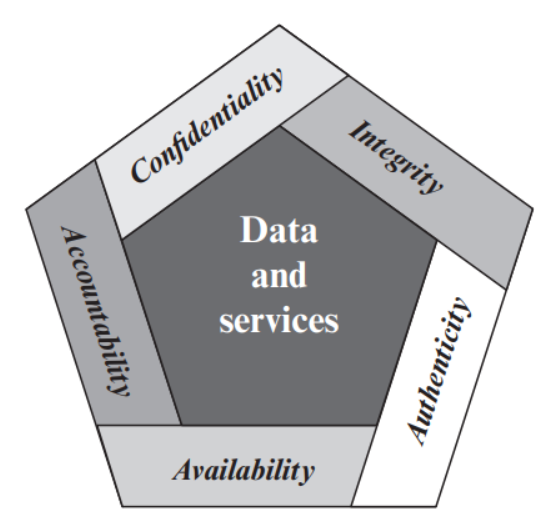
\includegraphics[width=\linewidth]{images/image-security.png}
    \caption{Essential Network and Computer Security Requirements.} \label{fig1}
\end{figure}

\subsubsection{Definicja kryterium oceny pod kątem skalowalności}

Czym jest skalowalność 

\begin{quote}
    "Scalability – the ability to work well when the load or the number of users increases – failure handling, concurrency of components, transparency and providing quality of service." ~\cite[p. 21]{coulouris2011distributed}
\end{quote}

W rozdziale 1 autorzy definiują pojęcie skalowalności jako 4 główne aspektu systemu Controlling the cost of physical resources, Controlling the performance loss, Preventing software resources running out, Avoiding performance bottlenecks, strony 20-21, czyli Kontrola kosztów zasobów fizycznych, Kontrola utraty wydajności, Zapobieganie wyczerpywaniu się zasobów oprogramowania, Unikanie wąskich gardeł wydajności, dlatego mogę zdefiniować kryterium oceny pod kątem skalowalności jako:

Wpływ na koszty zasobów fizycznych - ocena tego, jak wybrane podejście wpływa na  wykorzystaniem zasobów sprzętowych w miarę wzrostu obciążenia.

Wpływ na wydajność - ocena tego, jak wybrane podejście wpływa na wydajność systemu w miarę wzrostu obciążenia.

Wpływ na zasoby serwera - ocena tego, jak wybrane podejście wpływa na jakość wykorzystania zasobów serwera w miarę wzrostu obciążenia.

Unikanie wąskich gardeł wydajności - ocena tego,czy wybrane podejście powoduje powstanie wąskich gardeł  w miarę wzrostu obciążenia systemu.

\subsubsection{Definicja kryterium oceny pod kątem wersjonowania}

Za pomocą żrudeł literaturowych oraz własnego doświadczenia zdefiniowałem kryteria oceny pod kątem wersjonowania jako: 

\begin{enumerate}
    \item Kompatybilność wsteczna - Zapewnienie, że starsze wersje systemu lub komponentów nadal będą działały poprawnie, mimo wprowadzania nowych wersji. Kompaty bilność wsteczna pomaga zapełnić funkconowanie istniejących sytemów mikroserwisów w trakcie wproadzenie zmnian i rozwoju systemu, pozwala pszejść z kosztownych i bardzoi skomplikowanych upgradów systemu w całości za raz a podzielić prace na mniejsze, łatwiejsze do zarządzania kawałki.
    \begin{quote}
        "APIs, like diamonds, are forever. Once you publish an API, you are more or less stuck with it, so it is critically important to design it well. When evolving an API, preserving backward compatibility is crucial to avoid breaking existing clients." ~\cite[p. 75]{bloch2018effective}
    \end{quote}
    \item Łatwość migracji - Prostota przescia między wersjami, umożliwienie łatwego przechodzenia między różnymi wersjami plików lub interfejsów, aby dostosować się do zmian bez wprowadzania zakłóceń w pracy systemu. Możliwość zmniejszenia przestojów aplikacji w trakie prac serwisowych i możliwość płynnego przejścia na nową wersję. Proste migracje przyspieszają proces rozwiju aplikacji i zmniejszają ilośc błędów.
    \begin{quote}
        "When evolving an API, it is essential to provide a smooth migration path for clients. Deprecating old functionality rather than removing it immediately allows developers to transition gradually without breaking their systems." ~\cite[p. 78]{bloch2018effective}
    \end{quote}
    \item Zarządzanie historią wersji - Możliwość przechowywania i uzyskiwania dostępu do poprzednich wersji plików. Historia wersji pozwala programistom szybko i łatło przywrucić popradnią wersj w przypadku powstania błędu w nowej wersji. Pozwala na zmniejszenie uraty danych i niespówjnoscie w trakcie rozwoju aplikacji. Posiadanie historii versji zapewnia to, że projekty pozostaja łatwe w utrzymaniu i skalowalne.
    \begin{quote}
        "Effective version management is crucial for tracking changes over time, allowing teams to understand what was modified, when, and by whom. A well-maintained version history ensures accountability and facilitates rollback if necessary." ~\cite[p. 150]{rubin2012essential}
    \end{quote}
    \item Śledzenie zmian - Zdolność systemu do rejestrowania i monitorowania wszystkich zmian. Możliwość śledzenia zmian zapełnia to, że każda zmiana w systemie będzie zapisana wsięraąc tym programistów w zrozwiązywianiu problemów i bagów albo pazwalając wyscofać zminy. Poprawia spówpracę między zespołami wykazujac kto kiedy i dlaczego wprowadzał zminay co ziękasza również opdowiedzialność. W brażach regulowanych prawem taka audutowalność systemu może vyć wymagana przez prawo. 
    \begin{quote}
        "Tracking changes in source code is essential for understanding the evolution of a system. Without a proper change history, debugging, auditing, and maintaining software become significantly more difficult." ~\cite[p. 150]{rubin2012essential}
    \end{quote}
\end{enumerate}

\subsection{Ocena i porównanie metod współdzielenia kodu}

\subsubsection{Ocena wspówdzieleina kodu za pomocą Interface definition languages}

Ocena pod kątem komunikacji – zapewnia potrzebny poziom komunikacji, obiekty są generowane na podstawie definition language na etapie uruchamiania aplikacji, dalej w trakcie wykonania logiki programu takie obiekty mogą być użyte przez program bez żadnych obciążeń wydajnościowych. Obiekty wygenerowane z plików IDL mogą być wykorzystane dla komunikacji asynchronicznej takich jak brokery wiadomości jak również dla wysłania bezpośrednich zapytań między serwisami.

Metody zarządzania plikami idl w systemach : 

\begin{enumerate}
    \item SVN systemy takie jak, na przykład GIT - Rozwiaania posiada następujące korzyści: łatłe osiągniecie wstecznej kompatybilności, uałienie osiądgniecia jednego źrówdła prawdy w systemie mikroserwisów, łatwnie zapełnienienie tego że wsystrkiwe usługi korzystają z najnowszej wersie IDL. Do minusów rozwiazania możemy odnieść to, że system SVN może szybko stac wąskim gardłem w przypadku wykorzystania przez wilesepołów, wymaga zarządzania i utrzymania.
    \item Dystrybucja za pomocą bibliotek - Kompilowanie plików IDL do współdzielonych bibliotek, i publikacja w współdzielonym repozytorium pakietów, na przykład nexus. Do korzyście tego rozwiązani możemy oniść łatwą integrację c spocesami CI/CD, mozliwość orzystania z wersjonowanych artefaktów bez bezpośredniej interakcji z surowymi plikami IDL oraz to że różne języki programowania mogą wymagać różnych bibliotek, co zwiększa złożoność systemu.
    \item Podejście Monorepo - Przechowywanie wszystkich mikroserwisów i powiązane z nimi pliki IDL w jednym repozytorium, co zapewni, że wszystkie zespoły będą pracować na tej samej bazie kodu. Do korzysci tego rozwiazania możemy odnieść to, że pliki IDL w implementacja usług są zawsze zsynchronizowne oraz to, że takie podejście upraszcza rarządzanie zależnościami, poniważ cału kod przechowywany w jednym miejcu. Do wad podejscia mogę odnieść problemy ze skalowalnością zwiększenia ilości kodu oraz to, że często wymaga narzędzi do zarządzania dużymi bazami kodu.
    \item Repozytoria z automatyczną synchronizacją - Repozytoria z automatyczną synchronizacją to specyficnzy rodzaj repozytoriów, w których zmiany wprowadzone w głównym repozytorium są automatycznie propagowane do posoztałych sybrepozytoriów. Dzięki temu każdy uczestnik projektu ma dostęp do wszystkich wersji kodu. Do zalet tego podejścia możemy zaliczyć moźliwośc scentralizowanego wymuszania wersjonowania oraz łatwy dostęp do wszyskich wersji plików. Do minusów mozemy zapisać dość trudne utrzymianie oraz złożonosć w zarządzaniusynchronizacją i konfliktami w repozytorium.
    \item IDL as a Service (IDLaS) - Przygotowania wcieśniej usługa, która obsługuje pliki IDL na żądanie. Ta usługa może wersjonować, weryfikować i dostarczać pliki IDL. Do korzyście tego podejśćia możemy odnieść dostęp nazoądanie do plikow IDL, możliwośći dynamiczneg o wersjonowania. Do minusów możemy doliczyć ro, że takie podejście wymaga zbudowania i urzymnia dodatkowej usługi w systemie oraz to, że komunikacja śieciowa może powodoiwac opóźnienia w dostarczeiu plików IDL.
\end{enumerate}

Ocena pod kątem izolacji - ocena pod kątem izolacji zależy od implementacji, dla każdej z powyżej opisanych implementacji dokonałem analizy.

Ze wsględu na to, że mamy wiele kryteriów oceny i wiele mozliwych dodejść do współdzielenia plików IDL, postanowiełem stworzyć tabelę porównawczą, która pomoże w czytelnym preentowaniu wyników analizy i porównania.

Dane do porównania zostały zebrane z żródeł literaturowych ~\cite{newman2015building} ,  ~\cite{kleppmann2017designing}

\begin{table}[htbp]
    \centering
    \caption{Comparison of Code Sharing Approaches in Microservices}
    \label{tab:comparison}
    \begin{tabularx}{\textwidth}{|>{\raggedright\arraybackslash}X|>{\raggedright\arraybackslash}X|>{\raggedright\arraybackslash}X|>{\raggedright\arraybackslash}X|>{\raggedright\arraybackslash}X|>{\raggedright\arraybackslash}X|}
    \hline
    \textbf{Kryteria} & \textbf{SVN/Git Systemy} & \textbf{Biblioteki} & \textbf{Podejssćie Monorepo} & \textbf{Repo z Auto-Synchro.} & \textbf{IDL as a Service (IDLaS)} \\
    \hline
    \textbf{Conflict Rate} &
    Wysoki: Merge konflikty są powszechne w przypadku wykorzystanie przez kilkoma zespowani jednocześnie. Rozwiazanie takich konflików może być zasochłonne &
    Umiarkowany: Konflikty są mniej powszechne, ale wciaż moga wystapić. &
    Niski: Zespoły pracują na tej samej bazie kodu, dlatego konflikty zdarają sie rzadko, mogą wystqapic w trzyaku pracy na tej samej usłudze. &
    Umiarkowany: Konflikty mogą wystąpić, dlatego w przypadku gdy synchonizacja między usługami nie jest dobrze zarządzana. &
    Niski: Konflikty zdarzają się rzadko, dlatego, że IDL są dostarczne na rżadanie a wersjowaniee jest wymuszane. \\
    \hline
    \textbf{Version Drift Occurrence} &
    Umiarkowana: Może wystąpić jescli zespoły programistów nie aktualizują się do nowszej wersji regularnie. &
    Niski: Warygodność jest minimalna, poniewaz bibioteki sąa wersjonowane i dystrybuowane za pomocą odpowiednich narzędzi. &
    Niski: Bazy kody w tym przypaku baza kodu jest synchronizowana co minimalizyje problemy z wersjonowaniem. &
    Umiarkowany: Problemy moga wystąpić, jeśli synchronizacja nie jest dobrze utrzymana. &
    Bardzo Niski: Dynamiczna zarządzanie wersjami po stronie usługi zmniejsza Warygodność problemów z wersjonowaniem. \\
    \hline
    \textbf{Build Failure Rate} &
    Wysoki: Błędy w trakcie kompilacji pogą wystąpić w przypadku niekompatybilnych usług. &
    Umiarkowana: Awarie zrdarzają się rzadko, mozliwe są z przydaku nieprawidłowych wersji zawartych w bibliotece. &
    Umiarkowana: Błędy w trakcie kompilacji zadarzają się rzadko, ze względu na szynchronizację kodu. &
    Umiarkowana: Błędy w trakcie kompilacji zadarzają się rzadko, mozliwe w przypadku dysynchronizacji repozytorium. &
    Niska: Minimale ryzyko błędów w trakcie kompilacji ze wszledu na wymuszaną synchronizację. \\
    \hline
    \textbf{Deployment Rollback Frequency} &
    Wysoka: Zęste zminay w plikach IDL mogą spowodować częste wycofanie zmian w trakcie wdrożenia. &
    Umiarkowana: Wycofania zmian w trakcie wdrożenia mogą wystąpić, jeśli wystąpią problemy z kompatybilnością wsteczną. &
    Umiarkowana: Wycofania zmian w trakcie wdrożenia są rzadsze ze względu na synchronizację, ale problemy mogą wystapić. &
    Niska: Wycofania zmian w trakcie wdrożenia są rzadkie, automatyczna synchronizacja minimalizuje potrzebę wycofywania zmian. &
    Niska: Wycofania zmian w trakcie wdrożenia są rzadkie Zarządzanie IDL na żądanie zmniejsza częstotliwość wycofywania. \\
    \hline
    \end{tabularx}
\end{table}

\newpage

Ocena pod kątem bezpieczeństwa:

\begin{longtable}{|p{4cm}|p{4cm}|p{4cm}|}
\caption{Sample Longtable Caption} \\
\hline
\textbf{Criterion} & \textbf{Advantages} & \textbf{Challenges} \\ \hline
\multicolumn{3}{|c|}{\textbf{SVN (Subversion)}} \\ \hline
Confidentiality & Advanced access control mechanisms ensure confidentiality & Requires proper configuration to prevent unauthorized access \\ \hline
Integrity & Full change history ensures data integrity & Integrity issues can arise if changes are not properly synced \\ \hline
Availability & Central repository accessible from multiple locations & Central server failure may disrupt availability \\ \hline
Authenticity & User authentication controls access to the repository & Misconfigured authentication may lead to security issues \\ \hline
Accountability & Full change history allows attribution of actions & Auditing process must be properly configured \\ \hline
\multicolumn{3}{|c|}{\textbf{GIT}} \\ \hline
Confidentiality & Strong access control mechanisms in private repositories & Security configurations must be properly managed \\ \hline
Integrity & SHA-1 hashing ensures file integrity & Conflicts can arise if changes are not synchronized \\ \hline
Availability & Distributed system ensures high availability & Requires proper synchronization infrastructure \\ \hline
Authenticity & Supports authentication via SSH, HTTPS, and keys & Weak passwords or missing 2FA may pose risks \\ \hline
Accountability & Complete change history ensures tracking & Auditing in multi-user environments can be complex \\ \hline
\multicolumn{3}{|c|}{\textbf{Distribution via Repositories (Nexus, Artifactory)}} \\ \hline
Confidentiality & Authentication and access control protect IDL files & Improper security settings may lead to unauthorized sharing \\ \hline
Integrity & Version control and artifact signing ensure integrity & Lack of versioning or signing may cause issues \\ \hline
Availability & Central storage for artifacts ensures availability & Requires strong infrastructure for reliability \\ \hline
Authenticity & Signing mechanisms confirm trusted sources & Requires proper configuration to prevent forgery \\ \hline
Accountability & Auditing and monitoring track user actions & Proper logging is needed for accountability \\ \hline
\multicolumn{3}{|c|}{\textbf{Monorepo Approach}} \\ \hline
Confidentiality & Centralized access control improves security & Managing access in large repositories is complex \\ \hline
Integrity & Centralized changes ensure consistency & Synchronization challenges in large teams \\ \hline
Availability & Central repository allows easy access & Requires strong infrastructure for large-scale usage \\ \hline
Authenticity & Organizational-level access control ensures security & Managing permissions across large teams is difficult \\ \hline
Accountability & Centralized process allows full change tracking & Harder to attribute responsibility in large organizations \\ \hline

\end{longtable}

Ocena pod kątem skalowalności:

Systemy bazujące na IDL, taie jak Protocol Buffers oraz Avro zazwyczj sarilizują dane do kompaktowych formatów binarnych, to znaczy, że ilośc danych które trzeba przesłac przez sieć i przechowywac na dysku jest minimalna. Dzieki temu koszt zasobów fizycznych jest minimalny i ma tendencje do pozostania nizkim nawet w przypadku wzrostu obciążenia. Wydajność systemu kożystającego z wspówdzielenia za pomocą IDL nie zależy od metody zarządazania plikami IDL jak w powyzwych przypadkach.

\begin{quote}
    "With efficient binary serialization formats, IDLs allow rapid encoding and decoding of messages. This efficiency is crucial for high-throughput systems where low latency is required. IDLs also facilitate cross-language interoperability without incurring significant performance penalties." ~\cite[p. 123]{kleppmann2017designing}
\end{quote}

Ocena pod kątem wersjonowania:

Na podstawie analizy żródeł literaturowych oraz doświadczenia włąsnego dokonałem analizy podejścia do wpółdzielenia kodu za pomocą plików IDL. W tym trzybaku ocena pod kątem wersjonowania rówżni się w zależnosci od podejścia do zarządzania plikamu IDL, dlatego dokonałem porównania dla każdego z podejść.

\begin{longtable}{|C{3cm}|C{9.1cm}|}
    \caption{Sample Longtable Caption} \\
    \hline
    \textbf{Zaleta} & \textbf{Opis} \\
    \hline
    \endfirsthead

    \hline
    \textbf{Zaleta} & \textbf{opis} \\
    \hline
    \endhead

    \hline
    \endfoot

    \hline
    \endlastfoot

    \multicolumn{2}{|c|}{\textbf{1. SVN Systems (e.g., Git)}} \\ \hline
    Granular Tracking &
    \begin{itemize}
      \item Every change is recorded as a commit with messages, timestamps, and author information.
      \item Branching and tagging enable isolated development and marking of stable releases.
      \item The full commit history supports code reviews and audits.
    \end{itemize} \\ \hline
    Granular Tracking &
    \begin{itemize}
      \item Every change is recorded as a commit with messages, timestamps, and author information.
      \item Branching and tagging enable isolated development and marking of stable releases.
      \item The full commit history supports code reviews and audits.
    \end{itemize} \\ \hline

    \multicolumn{2}{|c|}{\textbf{2. Distribution via Libraries}} \\ \hline
    Semantic Versioning &
    \begin{itemize}
      \item Artifacts are assigned version numbers (MAJOR.MINOR.PATCH).
      \item Release notes and changelogs accompany each version.
      \item Central repositories maintain a full history of published versions.
    \end{itemize} \\ \hline

    \multicolumn{2}{|c|}{\textbf{3. Monorepo Approach}} \\ \hline
    Unified Change Log &
    \begin{itemize}
      \item All microservices and their associated IDL files reside in a single repository.
      \item A unified commit history provides a holistic view of changes.
      \item Synchronization minimizes version drift.
    \end{itemize} \\ \hline

    \multicolumn{2}{|c|}{\textbf{4. IDL as a Service (IDLaS)}} \\ \hline
    Integrated Version Control &
    \begin{itemize}
      \item The service includes built-in version control that tracks every change.
      \item Dashboards display diffs and metadata (timestamps, authors).
      \item Version history is accessible via standardized API calls.
    \end{itemize} \\ \hline

\end{longtable}

\subsubsection{Ocena wspówdzieleina kodu za pomocą bibliotek}

Ocena pod kątem komunikacji:

Pod kątem komunikacji podejście zapewnia potrzebny poziom komunikacji, obiekty są dodawane do projektu przez narzędzie do budowania projektów na etapie uruchamiania aplikacji, dalej w trakcie wykonania logiki programu takie obiekty mogą być użyte przez program bez żadnych obciążeń wydajnościowych. Obiekty wciągnięte z biblioteki mogą być użyte dla komunikacji asynchronicznej takich jak brokery wiadomości jak również dla wysłania bezpośrednich zapytań między serwisami.

Ocena pod kątem izolacji:

Zgodnie z wcieśniej zaprezentowanymi kryteriami oceny, w przypadku oceny izolacji bibliotek kryteria oceny są następujące: ocena pod kątem zolacji interfejsów, isolacja wersji, izolacja zależności.

Izolacja interfejsów: Biblioteki, złykle udostępniają zdefiniowany interfejs. Dobrze ustrukturyzowana biblioteka izoluje skonmlipkowane elementy logiki od swoich użytkowników. Gdy są użyte prawidłowo, pozwalają na zmianę lub aktualizację kodu przy minimalnym wpływie na kod wykorzystujący bibliotekę.

\begin{quote}
    "A well-designed library or SDK isolates its implementation details from the user." ~\cite[p. 75]{Essential}
\end{quote}

Izolacja wersji: Bibliotelki zazwycaj używają semantycznego wersjonowania za pomocą nazwy. Przejrzysta historia wersji umożliwia deweloperom odpowiednie zarządzanie zależnościami. Przy odpowiedniej izolacji wersji wiele wersji biblioteki może współistnieć i być używane jednocześnie, ułatwia to sproces stopniowej migracji.

\begin{quote}
    "Versioning APIs and libraries carefully ensures that changes can be introduced gradually." ~\cite[p. 172]{fowler2012patterns}
\end{quote}

Izolacja zależności: Biblioteki często zależą od innych bibliotek, w przypadku gdy zależności nie są prawidłowo izolowane mogą prowadzić do konfliktów i innych problemów. Dobre praktyki zarządzania zależnościami pomagają zapewnić, że zależności biblioteki nie będą miały negatywnego wpływu na aplikację.

\begin{quote}
    "Dependencies should be isolated to minimize their impact on the main application." ~\cite[p. 218]{martin2008clean}
\end{quote}

Ocena pod kątem bezpieczeństwa:

Zgodnie z wcieśniej zaprezentowanymi kryteriami oceny, w przypadku oceny bezpieczeństwa bibliotek kryteria oceny są następujące: Poufność, Integralność danych, Dostępność, Autentyczność, Odpowiedzialność

Poufność: Biblioteki które są wykorzystywane dla preteażania poufnuch danych powinny pochodzić z sprawdzonych żródeł i ciągle aktualizowane aby zapobiec utratę danych. Ich integracja powinna wymuszać ścisłe kontrole dostępu. 

\begin{quote}
    "Ensuring that libraries handling sensitive information are sourced from reputable channels and regularly updated is critical to maintaining confidentiality throughout an application." ~\cite[p. 82]{Essential}
\end{quote}

Integralność danych: Biblioteki często korzystją z sum kontrolnych, certyfikatów, podpisów cyfrowych przeprowadzają obszerne testy, aby mieć pewność, że przetwarzane dane pozostają biezpieczne.

\begin{quote}
    "The integrity of a library is maintained through rigorous testing and the use of cryptographic measures that detect any unauthorized changes to the code or data it processes." ~\cite[p. 84]{Essential}
\end{quote}

Dostępność: Dostępność może zostać naruszona, jeśli biblioteki zewnętrzne staną się nieobsługiwane lub niedostępne lub wewnętrzne w przypadku awarii narzędzia do zarządzania bibliotekami. Dlatego jest ważnym wykożystanie managarów zależności które są zaufane i w tym przupadku możemy pomaga zapewnić, że aplikacje pozostaną dostępne nawet w miarę ewolucji bibliotek.

\begin{quote}
    "By leveraging modern dependency management tools and regularly updating libraries, developers can mitigate risks to availability due to deprecated or unsupported components." ~\cite[p. 85]{Essential}
\end{quote}

Autentyczność: W przypadku bibliotek jest zapewniania za pomocą sprawdznie jej pochodzenia za pomocą podpisów cyfrowych i sum kontrolnych dostarczonych przez wydawcę. Zapobiega to ryzyku włączenia wykonania złośliwego kodu po stronie klienta biblioteki. 

\begin{quote}
    "Authenticating libraries through digital signatures and secure distribution channels is essential to ensuring that only verified, unmodified code is used in production environments." ~\cite[p. 87]{Essential}
\end{quote}

Odpowiedzialność: W pzypadku bibliotek przejrzysta historia mnoże zostać zapełniona za pomocą menedżerów pakietów które umożliwiają śledzenie pochodzenia zmian. Wspomaga to w zabiezpieczniu odpowiedzialności w przypadku problemów.

\begin{quote}
    "A well-documented version history is indispensable for accountability, as it enables developers to trace and audit every modification made to a library over time." ~\cite[p. 88]{Essential}
\end{quote}

Ocena pod kątem skalowalności:

Libraries are generally optimized for specific tasks within one language. However, if a library is not designed for high-concurrency environments, it may require additional hardware resources as the load increases. For example, intensive data processing libraries may consume more memory or CPU when dealing with large datasets. Supporting Idea: Studies on computational efficiency often note that non-optimized libraries can become bottlenecks under heavy load, leading to increased physical resource costs.

\begin{quote}
    "Non-optimized libraries can quickly become bottlenecks in high-concurrency environments, forcing systems to consume additional CPU and memory resources as load increases." ~\cite[p. 192]{fowler2012patterns}
\end{quote}

Ocena pod kątem wersjonowania:

\begin{quote}
    "When a data format or schema changes, … careful management of schema evolution is required to ensure that old and new versions can coexist. This is best achieved by maintaining a structured version history that records every change in the schema in a clear, traceable manner." ~\cite[p. 111]{kleppmann2017designing}
\end{quote}

Ustrukturyzowana historia wersji:

\begin{quote}
    "APIs, like diamonds, are forever. Once you publish an API, you are more or less stuck with it; hence, maintaining a clear, structured version history through semantic versioning is critical for ensuring that developers know exactly when breaking changes occur." ~\cite[p. 75]{Essential}
\end{quote}

text

\begin{quote}
    "When an API change turns out to be problematic, having a stable version available through semantic versioning allows developers to quickly roll back to a previous release and restore system stability." ~\cite[p. 75]{Essential}
\end{quote}

text

\begin{quote}
    "Inadequate versioning can lead to subtle incompatibilities, resulting in data inconsistencies that are difficult to debug. Hence, maintaining strict backward compatibility is crucial to avoid such pitfalls." ~\cite[p. 75]{Essential}
\end{quote}

\subsubsection{Ocena wspówdzieleina kodu za pomocą SDK}

Ocena pod kątem komunikacji: zapewnia potrzebny poziom komunikacji, mechanizm współdzielenia jest podobny do biblioteki, tak samo jak w przypadku biblioteki obiekty są dodawane do projektu przez narzędzie do budowania projektów na etapie uruchamiania aplikacji, dalej w trakcie wykonania logiki programu takie obiekty mogą być użyte przez program bez żadnych obciążeń wydajnościowych. Obiekty wciągnięte z biblioteki mogą być użyte dla komunikacji asynchronicznej takich jak brokery wiadomości jak również dla wysłania bezpośrednich zapytań między serwisami.

Ocena pod kątem izolacji: 

Zgodnie z wcieśniej zaprezentowanymi kryteriami oceny, w przypadku oceny izolacji SDK kryteria oceny są następujące: ocena pod kątem zolacji interfejsów, isolacja wersji, izolacja zależności. Jednak są one trudniejsze w projetowaniu i wymagają strrności w trakcie trzygowania.

\begin{quote}
    "SDK isolates its implementation details from the user, allowing developers to interact with the API without needing to understand its inner workings." ~\cite[p. 75]{Essential}
\end{quote}

Izolacja wersji: W przypadku SDK które agregują kilka bibliotek i narzędzi muszą zarządzać werjsjonowanie wszystkicjh zawartych komponentów. W idealnym przypadku zestaw SDK jest zaprojektowany tak, aby nowe dodane wersje byli kompatybilne wstecz umożliwiając klientom działanie bez natychmiastowych zmian.

Izolacja zależności: SDK często zawerają wiele biblioter w spobie, co oznacze że często zarządzają wilką ilością zależności. Izolowanie tych zależności jest krytyczne, aby uniknąć konfliktów.

\begin{quote}
    "...ensuring that dependencies can be replaced without affecting the core business logic" ~\cite[p. 218]{martin2008clean}
\end{quote}

Ocena pod kątem bezpieczeństwa: 

Zgodnie z wcieśniej zaprezentowanymi kryteriami oceny, w przypadku oceny bezpieczeństwa bibliotek kryteria oceny są następujące: Poufność, Integralność danych, Dostępność, Autentyczność, Odpowiedzialność

Poufność: SDK w przypadku polączenia wielu narzędzi i bibliotek, muszą zapewnić, że wszystkie zawarte komponenty przestrzegają ścisłych zasad kontroli dostępu. Zmniejsza to ryzyko nieautoryzowanego ujawnienia danych.

\begin{quote}
    "SDKs, when integrated with stringent access controls and privacy policies, help shield sensitive data from unauthorized access, thus preserving confidentiality across all integrated modules." ~\cite[para 4]{azure2020}
\end{quote}

Integralność danych: SDK wymaga, aby były one kompleksowo testowane, aby zapewnić, że zmiany nie naruszą integralności danych. Różne frameworki do testowania bezpieczeńswa SDK pomagają w wykrywaniu wszelkich podatności po modyfikacji.

\begin{quote}
    "Robust testing frameworks within SDKs are critical for maintaining integrity, ensuring that updates do not inadvertently alter data structures or application behavior." ~\cite[para 5]{azure2020}
\end{quote}

Dostępność: SDK muszą być zaprojektowane tak, aby działały zawszę, nawet przy dużym obciążeniu. 

\begin{quote}
    "The modular and redundant design of well-architected SDKs contributes significantly to system availability, ensuring that critical services remain accessible even under peak loads." ~\cite[para 6]{azure2020}
\end{quote}

Autentyczność: Autentyczność w przypadku z SDK może zostać zapewniona za pomocą weryfikacji dostawców i stosowanie środków kryptograficznych do walidacji ich komponentów. Warto dokonywac tachi wdziałań aby zapobiec wykonaniu złośliwego kodu w naszym systemie.

\begin{quote}
    "Verifying the authenticity of an SDK via cryptographic signatures and secure distribution channels is vital to ensure that the components used are genuine and have not been tampered with." ~\cite[para 7]{azure2020}
\end{quote}

Odpowiedzialność: SDK zazwyczaj posiadają przeróżne mechanizmy zarządzanie wersjami. Takie metody zarzadzania wersjami umożliwia deweloperom śledzenie pochodzenia wszelkich zmian lub problemów. Pomaga to zapełnić odpowiedzialność programistów za przygotowane zmiany.

\begin{quote}
    "Comprehensive logging and version tracking in SDKs provide the necessary audit trails that hold developers accountable for every change made, thereby ensuring that any issues can be traced back to their origin." ~\cite[para 7]{azure2020}
\end{quote}

\nocite{*}

\listoftables

\listoffigures

\bibliographystyle{plain}
\bibliography{thesisbibliography}

\section{Appendices}

\subsection{Sample Code}
\subsection{Sample Data}

\end{document}